\section{Risultati}\label{sec:risultati}
L'esecuzione dei test è stata effettuata su griglie quadrate di dimensione: 3, 4, 5, 6, 8, 10.
La dimensione massima della griglia è stata posta a 10 in quanto sia la codifica in MiniZinc che quella in ASP hanno mostrato il raggiungimento della soglia dei 300 secondi di esecuzione in tutte e 20 le griglie generate.

\begin{figure}
    \centering
    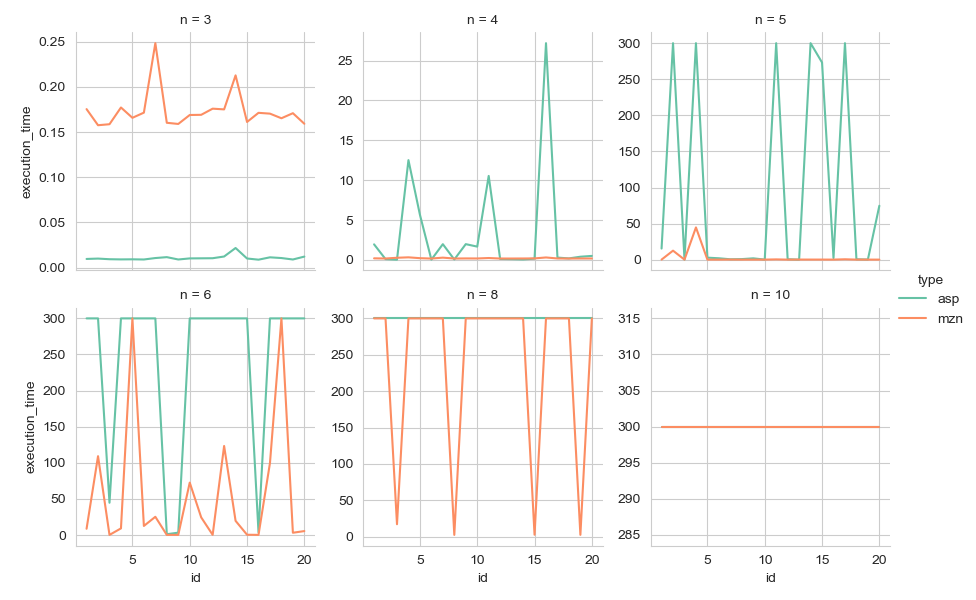
\includegraphics[width=0.8\textwidth]{img/cmpplot}
    \caption{Confronto tra ASP e MiniZinc}
    \label{fig:cmpplot}
\end{figure}

Come visibile dalla figura~\ref{fig:cmpplot}, la codifica in MiniZinc si è rilevata essere più performante rispetto a quella in ASP per le griglie di dimensione superiore a 3, con alcune eccezioni per le griglie di dimensione 4.

La codifica in ASP ha iniziato a saturare il tempo di esecuzione a partire dalla griglia di dimensione 5, mentre la codifica in MiniZinc ha iniziato a saturare il tempo di esecuzione a partire dalla griglia di dimensione 6.

\begin{figure}
    \centering
    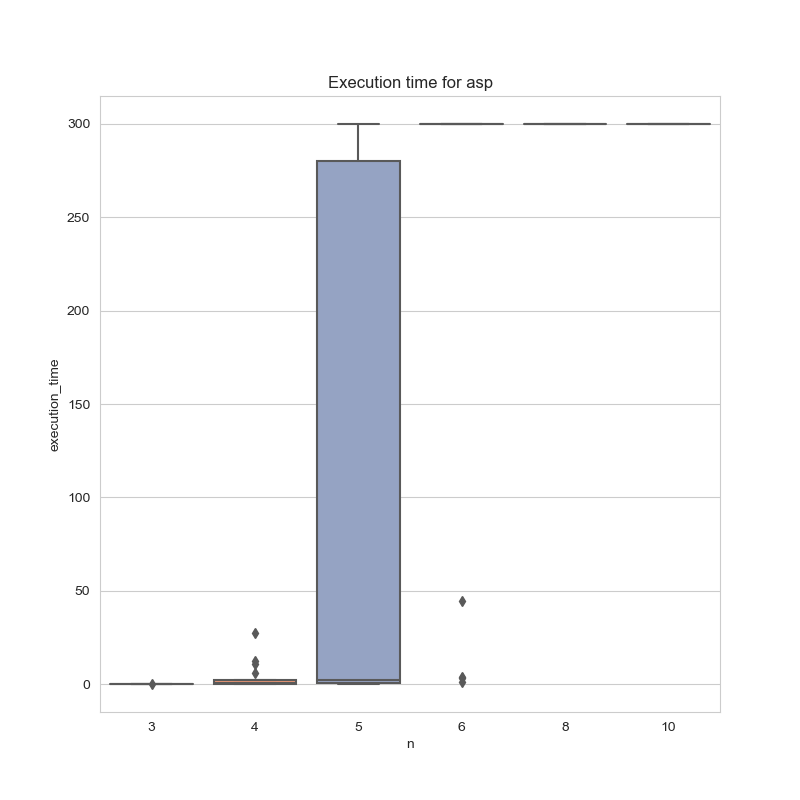
\includegraphics[width=0.5\textwidth]{img/boxplot_asp}
    \caption{Boxplot dei tempi di esecuzione in ASP}
    \label{fig:boxplot_asp}
\end{figure}

\begin{figure}
    \centering
    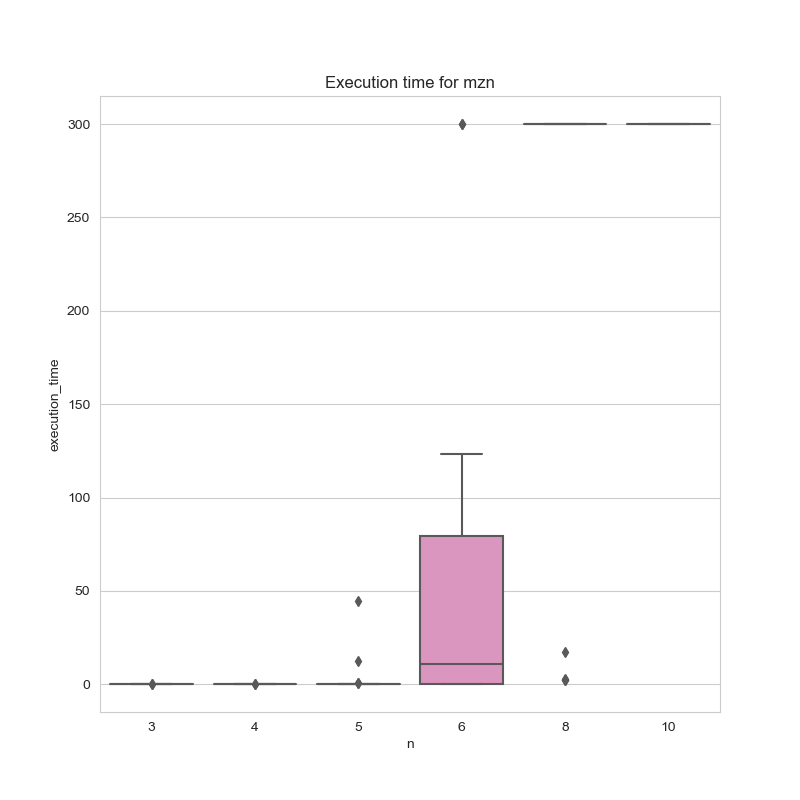
\includegraphics[width=0.5\textwidth]{img/boxplot_mzn}
    \caption{Boxplot dei tempi di esecuzione in MiniZinc}
    \label{fig:boxplot_mzn}
\end{figure}

I boxplot delle figure~\ref{fig:boxplot_asp} e~\ref{fig:boxplot_mzn} mostrano come la codifica in ASP sia meno stabile rispetto a quella in MiniZinc, in quanto i tempi di esecuzione sono molto meno concentrati attorno alla mediana (vedi griglia di dimensione 5 in ASP e griglia di dimensione 6 in MiniZinc).

È stato generato anche un grafico di correlazione per indagare la dipendenza tra il tempo di esecuzione e la dimensione della griglia, il numero di caselle occupate e il numero di caselle libere.

\begin{figure}
    \centering
    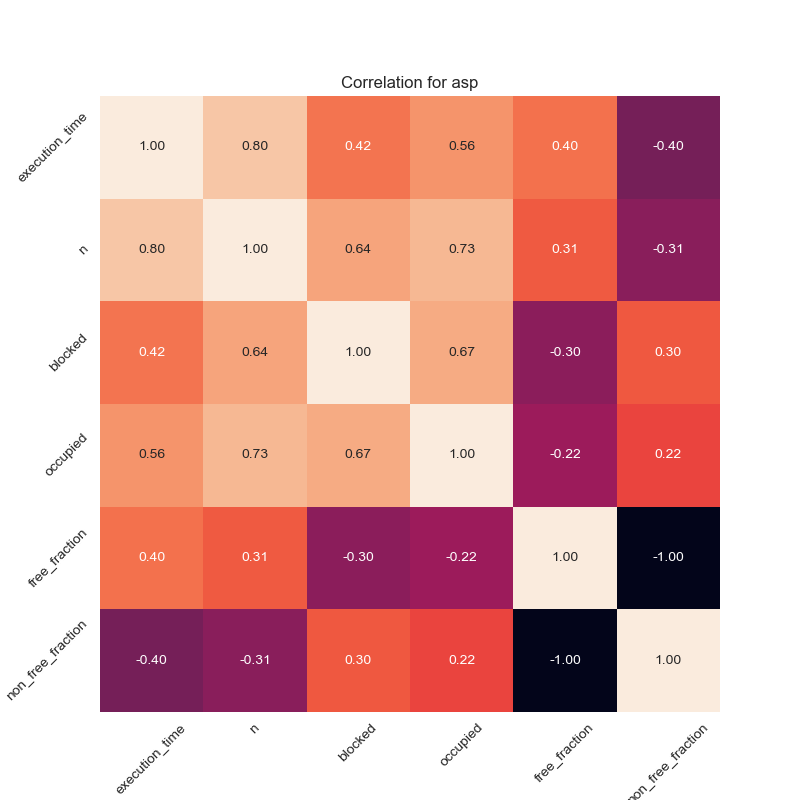
\includegraphics[width=0.5\textwidth]{img/correlation_asp}
    \caption{Grafico di correlazione per ASP}
    \label{fig:correlation_asp}
\end{figure}

\begin{figure}
    \centering
    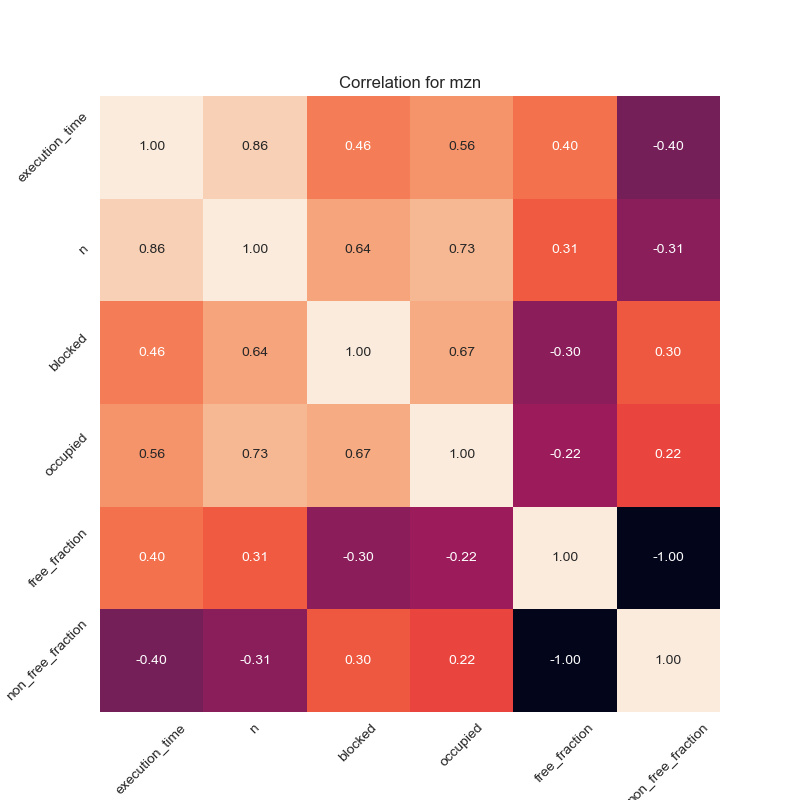
\includegraphics[width=0.5\textwidth]{img/correlation_mzn}
    \caption{Grafico di correlazione per MiniZinc}
    \label{fig:correlation_mzn}
\end{figure}

Come riportato in entrambi i grafici di correlazione (figure~\ref{fig:correlation_asp} e~\ref{fig:correlation_mzn}), il tempo di esecuzione è fortemente correlato con la dimensione della griglia, mentre c'è un moderato livello di correlazione con il numero di caselle occupate e il numero di caselle libere.
Questo può essere dovuto al fatto che aumentando la dimensione della griglia aumenta notevolmente il livello di difficoltà del problema mentre il numero di caselle occupate rimane una frazione (massimo 1/3) del numero di caselle totali.

A scopo di completezza, è stata creata una breve animazione che mostra una comparativa della risoluzione della griglia numero 15 di dimensione 5 nelle due codifiche proposte.
L'animazione è disponibile su YouTube al seguente \href{https://youtu.be/e243VU-qNLE}{indirizzo}.